\newpage
\section{Реализация}

% Если в рамках работы проводится реализация некоторого программного средства,
% то в разделе «Описание практической части» обязательно должна быть описана
% его программная реализация, в частности:
% приведены обоснования выбранного инструментария;
% приведена с иллюстрацией общая архитектура разработанного средства;
% приведена с иллюстрацией схема работы средства;
% если осуществляется доработка существующего средства, то должны быть описаны
% новые возможности/улучшения, реализованные в данной работе.
% обязательно должны быть приведены характеристики функционирования (например,
% сложность, производительность, время реакции и т.д.)
\subsection{Библиотека libsvm}
Библиотека libsvm содержит реализацию метода опорных векторов. Она содержит интерфейсы для построения моделей по обучающей выборки и предсказания значения целевой функции по  существующей модели. Дополнительно эта библиотека содержит интерфейсы для сохранения модели в файл и загрузки ее из файла.

Для создания модели можно пользоваться несколькими ядровыми функциями(линейная, полиномиальная, сигмоид и другие), а также задавать все необходимые для работы метода параметры.

Кроме того можно указывать тип решаемой задачи: классификация, классификация с двумя классами, регрессия и др.

Существует версия библиотеки libsvm использующая современные графические процессоры, логика работы в которой написана на CUDA. Использование графических процессоров позволяет существенно уменьшить время построения модели и время предсказания(смотри график).

Вместе с библиотекой поставляются некоторое количество исполняемых файлов, которые позволяют строить модель по данным из файла в определенном формате, а также осущесвлять предсказание для даннах записанных в файле по построенноей модели. Также поставляется некоторое количество тестовых данных.

\subsection{Архитектура dspam}
В основе dspam лежит библиотека libdspam, которая реализует логику фильтрации.
Эта библиотека содержит код нескольких алгоритмов фильтрации (одновременно использоваться может только один из них)
Кроме того библиотека содержит несколько вспомогательных классов реализующих некоторые структуры данных(списки, деревеья и т. п), а также драйвер хранилища данных.

Данные могут храниться либо в одной из поддерживаемых СУБД(это MySQL, Posgres и SQLite), а также непосредтсвенно в файловой системе(используется собственная методика хранения пар ключ-значение).

\begin{figure}[h]
\begin{center}
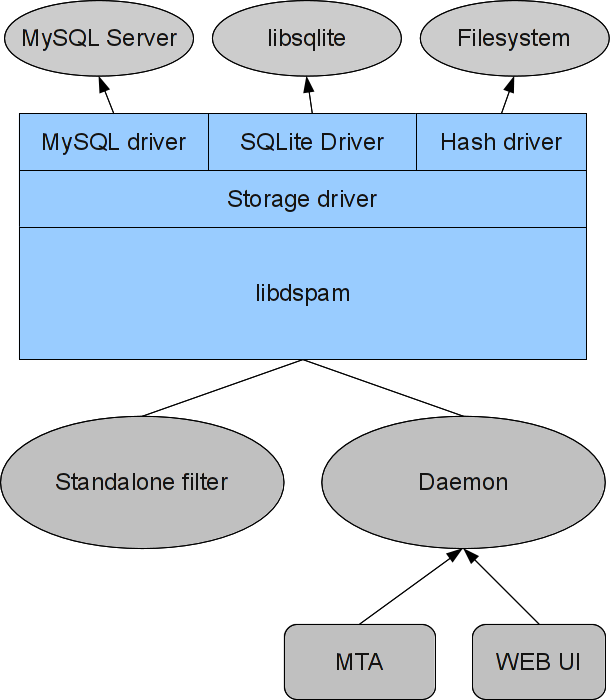
\includegraphics[width=10cm]{img/dspamarch}
\end{center}
\caption{Архитектура dspam}
\label{dspamarch}
\end{figure}

Dspam может работать либо в режиме standalone-фильтра, либо демона. В обоих случаях
исполняемый модуль линкуется с библиотекой libdspam.

Работа в standalone режиме подразумевает что бинарный файл запускается по требованию. Тестируемое письмо в этом случае подается исполняемому модулю на стандартный вход, а информацию о произведенном тестировании можно
получить со стандартного вывода. Эта информации может быть представлена в виде короткой строчки в которой содержится класс, к которому отнес классификатор письмо и вероятностью или в виде самого письма с установленными заголовками. Этот режим удобно использовать для тестирования системы, а так же в случае кода количество писем достаточно мало и требование к производительности невелики.

Работа в режиме демона подразумевает что исполняемый код постоянно находится в оперативной памяти. Общение с клиентом в этом случае происходит либо через сеть (используется tcp-сокет), либо через UNIX-сокет. Таким образом dspam в этом случае является полноценным серверным приложением. Сервер по запросу от клиента принимает письмо, классифицирует, проставляет необходимые заголовки и возвращает клиенту. Клиентом в таком случае выступает система доставки почты(MTA).

Кроме того сервер может выполнять некоторые сервисные команды: просмотр статистики, очистка хранилища данных и т. п. В этом случае клиентом может быть например web-интерфейс администратора.


\subsection{Модификация dspam}
Для обеспечения работы описанного в разделе \ref{research} метода была произведена модификация библиотеки libdspam: в функцию обработки письма был добавлен код, который при определенных настройках вызывает функцию обработки письма нашим методом.

Функция обработки обрабатывает уже разбитое на токены письмо. Для разбития письма на токены используется встроенная в dspam функциональность. В зависимости от режима работы(обучение или классификация) вызывается одна из двух функций.

Функция обучения записывает в файл информацию об адресате письма и частотах токенов. По этому файлу в последствии строится модель для метода опорных векторов

Функция классификации загружает из файла уже построенную модель, строит вектор с частотами и вычисляет вероятности.

\subsection{Схема работы}
Опишем схему работы разработанного средства в различных случаях.
\begin{figure}[h]
\begin{center}
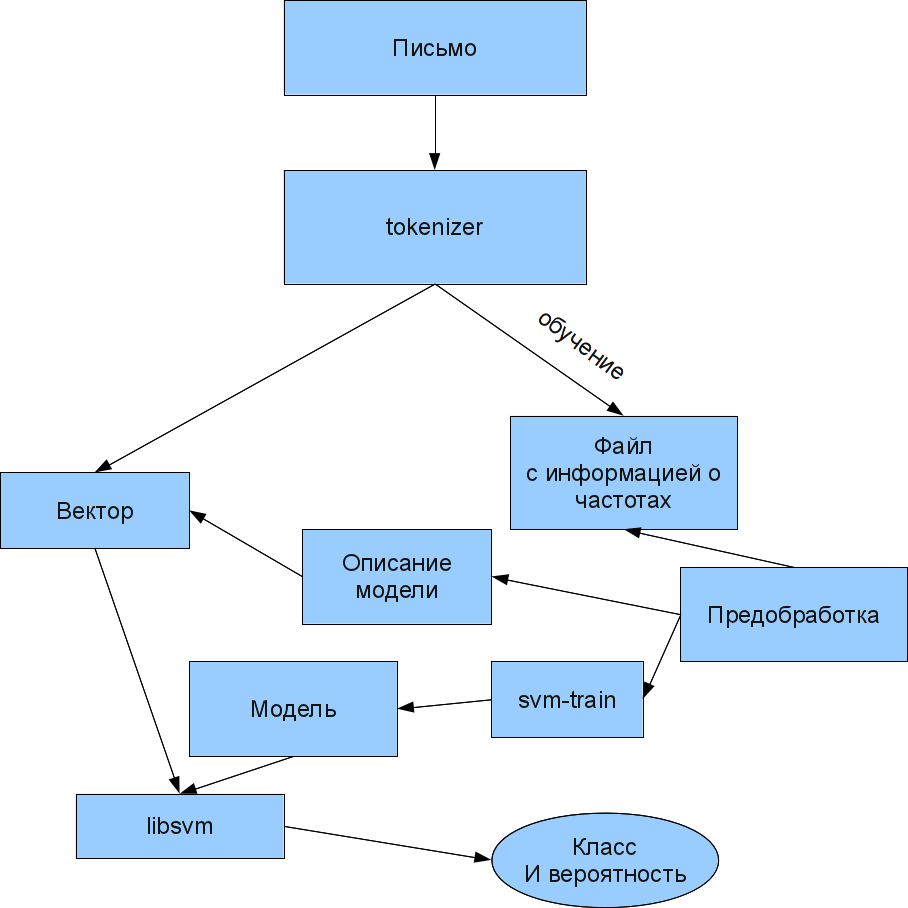
\includegraphics[width=12cm]{img/working_scheme}
\end{center}
\caption{схема работы классификатора}
\label{dspamarch}
\end{figure}

\subsubsection{Добавление письма в обучающую выборку}

\begin{enumerate}
    \item Письмо попадает в систему.
    \item Выясняется адресат письма.
    \item Письмо разбивается на токены.
    \item Вычисляются частоты токенов.
    \item Информация о классе письма, адресате и частотах токенов записывается в файл частот.
\end{enumerate}

\subsubsection{Построение модели}
\begin{enumerate}
    \item Вызывается скрипт построения модели (вызов происходит раз в день при помощи стандартной службы CRON).
    \item Вычисляются общие частоты токенов для каждого токена из файла частот.
    \item Выбираются наиболее употребимые токены (токены с наибольшей частотой).
    \item Для каждого из писем строится вектор, содержащий частоты наиболее употребимых токенов, а также индикаторы принадлежности письма пользователю (все кроме одного индикаторы равны нолю).
    \item Построенное множество векторов записывается во временный файл вместе с информацией о классах писем,  соответсвующих векторам.
    \item По построенному временному файлу генерируется модель при помощи инструмента svm-train.
    \item Информация о токенах используемых для построения модели сохраняется во временный файл описания модели.
\end{enumerate}

\subsection{Классификация}
\begin{enumerate}
    \item Письмо попадает в систему.
    \item Выясняется адресат письма.
    \item Письмо разбивается на токены.
    \item Вычисляются частоты токенов.
    \item Загружается описание модели
    \item По описанию модели, адресату и частотах токенов строится вектор
    \item Загружается модель
    \item По модели и вектору вычисляется вероятность принадлежности письма спаму
    \item По пороговому правилу выставляется оценка спам/не спам
\end{enumerate}

